
\subsubsection*{Preguntas tipo icfes matem\'aticas. Responda las preguntas \ref{vic-1} y \ref{vic-2} con base en la siguiente informaci\'on.}

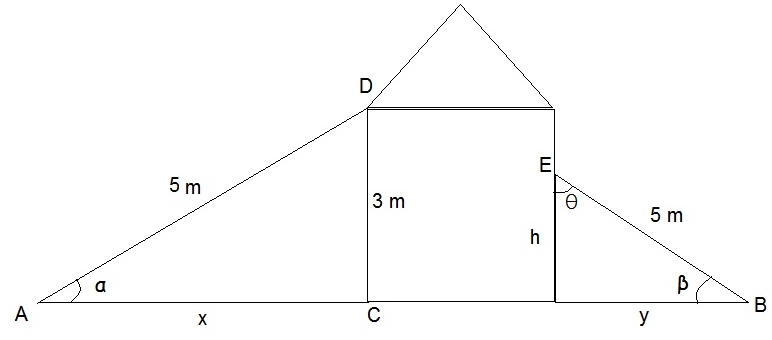
\includegraphics[width=0.45\textwidth]{vic_1_2.jpg}
%\centering\captionof{figure}{Preguntas \ref{vic-1} y \ref{vic-2}}\label{fig:vic-1-2}
%\justifying
\begin{enumerate}
\item En un paseo de grupo de estudiantes de grado 11$^o$, han armado una carpa que est\'a sujeta por dos cuerdas de 5 metros para darle mayor estabilidad. Tanto la cuerda A como la cuerda B  miden 5 metros y se sujetan de los puntos como se muestra. \label{vic-1}\\

La distancia x desde el punto A hasta el punto C es igual a:
\begin{enumerate}[(A)]
\item 8 m
\item 6 m 
\item 4 m 
\item 2 m
\end{enumerate}

\newpage
\item Si la cuerda B se sujeta de a la carpa a una altura h  y se sabe que el ángulo de elevación de la cuerda respecto a la horizontal es  $\beta$, entonces la altura h se puede expresar como:\label{vic-2}

\begin{enumerate}[(A)]
\item $5m x \sin\beta$
\item $5m x \cos\beta$
\item	$\frac{\sin\beta}{5}$
\item $\frac{\cos\beta}{5}$
\end{enumerate}
\item Un informe sobre el consumo de fruta de un grupo de niños durante la hora de descanso, lo hicieron de la siguiente \label{vic-3} manera:\\
50 comieron piña \\
40 - pera \\
30 - manzana\\
15 - ninguna\\
Pero debemos anotar que algunos comieron más de una fruta:\\
10 - piña y pera\\
5 - piña, pera y manzana\\
5 - piña y manzana\\
10 - pera y manzana\\
El número total de niños es:
\begin{enumerate}[(A)]
\item 80
\item 100
\item 120 
\item 135
\end{enumerate}


\begin{center}
\begin{table*}[htp]
%\begin{multicols}{1}
\begin{tabular}{|c|p{8.5cm}ccc|}
\hline 
PUESTO	&EDIFICIO	&PISOS	&ALTURA(m)	&AÑO\\
\hline \hline 
1	&Taipéi 101,Taipei(Taiwan)	&101	&509	&2004\\
2	&Petronas, Torres 1 Kuala Lumpur (Malasia)	&88	&452	&1998\\
3	&Petronas, Torres 1 Kuala Lumpur (Malasia)	&88	&452	&1998\\
4	&Torre Sears, Chicago (EE.UU)	&110	&442	&1974\\
5	&Edificio Jin Mao, Shanghai (China)	&88	&421	&1979\\
6	&Centro Int. de finanzas II, Hong Kong (China)	&88	&415	&2003\\
7	&Citic Plaza, Guangzhou (China)	&80	&391	&1996\\
8	&Shun Hing Square, Shenzhen (China)	&69	&384	&1996\\
9	&Edificio Empire State , New York (EE.UU)	&102	&381	&1931\\
10	&Central Plaza Hong Kong(China)	&78	&374	&1992\\
\hline 
\end{tabular} 
\captionof{table}{Tabla pregunta \ref{pregunta_altura}.}
%\end{multicols}

\end{table*}

\end{center}

\newpage


\item Se tiene la palabra impresiones, si se ponen en una bolsa cada letra y se saca una al azar, ¿cuál es la probabilidad de que la letra sacada sea una consonante? \label{vic-4} 
\begin{enumerate}[(A)]
\item $\frac{6}{11}$
\item $\frac{3}{11}$c
\item $\frac{1}{11}$
\item $\frac{8}{9}$
\end{enumerate}
\item El profesor Carlos pensando un ejercicio demora los 5/3 de un minuto; redactando el enunciado 4 minutos y 15 segundos; buscando los distractores 1/12 de hora y pasándolo a limpio 3 y $3/4$ de minuto.  ¿Qué tiempo empleó en elaborar 35 preguntas de una prueba de amptitud  matemática?\label{anexo_1}\label{vic-5}
\begin{enumerate}[(A)]
\item 12 h y 15 minutos.
\item 30.800 segundos.
\item 6.250 minutos.
\item 16 h. y 3 segundos.
\end{enumerate}



\item Antes  del siglo XIX, los edificios muy altos eran poco usuales, pero con la invención de diversos materiales como el acero y el hormigón, se hizo posible que iniciara la construcción de los primeros rascacielos. Desde su aparición hasta la actualidad, distintas potencias del mundo se han dado a la tarea de construir el edificio más alto del mundo. En este arduo proceso le han demostrado al mundo impactantes obras arquitectónicas. En la imagen se presenta una tabla con los datos de los 10 edificios más altos del todo el mundo.\label{vic-6} \label{pregunta_altura} \\

El edificio con menor altura por piso es:\hrulefill\\
\_\hrulefill\hrulefill\\
\_\hrulefill.

\item Se tiene un tanque cuya capacidad es de 32.480 litros. Está provisto de dos llaves: la llave A vierte 201 litros en 3 minutos. Y la llave B, 540 litros en 5 minutos; además tiene un desagüe C por el que escapan 240 litros en 8 minutos. El tiempo que tarda en llenarse del tanque, estando totalmente desocupada y abiertas las llaves y el desagüe, es: \label{vic-7}

\begin{enumerate}[(A)]
\item 3 h 44'
\item 3 h 68'
\item 4 h 33'
\item 4 h 73'
\end{enumerate}

\newpage
\item En las olimpiadas de matemáticas del Colegio Central se hacen 40 preguntas y cada pregunta correcta se premia con 5 puntos buenos; mientras que cada pregunta mal contestada se califica con tres puntos malos. Si contestando todas las preguntas el resultado es cero; las preguntas correctas fueron: \label{vic-8}
\begin{enumerate}[(A)]
\item 5
\item 15
\item 22
\item 25
\end{enumerate}
\item A un grupo de personas pertenecientes a un club de la tercera edad se le pregunto cuál era la actividad  que más le agradaba realizar sobre su permanencia en el club, de tres actividades posibles. Los resultados de la encuesta se presentan en la tabla que aparece en la imagen.\label{vic-9}

\begin{center}
\begin{tabular}{p{2cm}|p{1.8cm} p{2.5cm}}
\hline \hline 
Actividad	&Frecuencia Relativa	&Frecuencia\par relativa\par acumulada 	\\
\hline \hline 
Gimnasia	&12	&12	\\
Juegos de Mesa	&X	&W	\\
Leer	&9	&40	\\
\hline \hline 
\end{tabular} 
\end{center}

%\hrulefill\\
%\_\hrulefill\hrulefill\\
%\_\hrulefill.

\subsubsection*{Pregunta de selección múltiple con única respuesta. Responda con base en la siguiente información}

%\begin{flushleft}
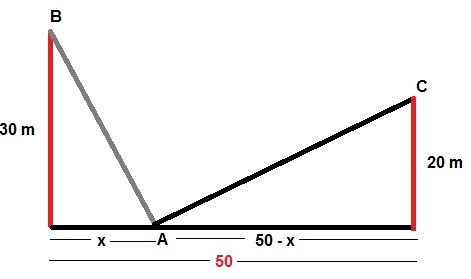
\includegraphics[width=0.45\textwidth]{vic_10.jpg} 
%\end{flushleft}
%\centering\captionof{figure}{Pregunta \ref{vic-10}}\label{fig:vic-10}
%\justifying

\newpage
\item Tenemos un poste de 30 metros de alturas y uno de 20 metros, la distancia entre ellos es de 50 metros. Se debe extender una cuerda que los une desde el extremo superior de cada uno de ellos. El centro de la cuerda debe tocar el piso. ¿a qué distancia del poste más bajo debe tocar el piso? \label{vic-10}\hrulefill\\
\_\hrulefill\hrulefill\\
\_\hrulefill.

%\begin{flushleft}

%\end{flushleft}
%\centering\captionof{figure}{Pregunta \ref{vic-11}}\label{fig:vic-11}
%\justifying
\item Se dice que una ventana es de estilo normando si tiene la forma de un cuadrado rematado por un semicírculo en la parte superior. Si r es el radio del semicírculo que está dada por $\frac{\pi r^2}{2}$  , y un cuadrado de radio $2r$, cuya área es igual a lado por lado, según la información suministrada el área de la ventana está dada por: \label{vic-11}

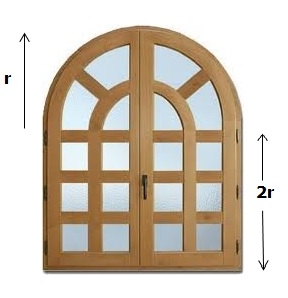
\includegraphics[width=0.45\textwidth]{vic_11.jpg} 

\begin{enumerate}[(A)]
\item $\frac{1}{4}r^2\pi+2r^2$
\item $\frac{\pi r^2}{2}+4r^2$
\item $r^2\pi+2r^2$
\item $\frac{1}{2}\pi+4r^2$
\end{enumerate}

\newpage
\subsubsection*{Pregunta de selección múltiple con única respuesta. Responda de acuerdo con la siguiente información}
\item Se realiza una convocatoria para unas vacantes en un circo y quedan seleccionado de la siguiente manera  hay 32 artistas, de estos 16 bailan, 25 cantan y 12 cantan y bailan. Según esto se desea saber el número de artistas que se incorporaron al circo que  no  cantan y bailan \label{anexo_conjuntos}\label{vic-12} 

\begin{enumerate}[(A)]
\item 10
\item 5
\item 8
\item 3
\end{enumerate}
\item En el curso de noveno  hay 30 estudiantes el 55\% tiene una nota en superior, el 35\% tiene notas en básico y el resto de las notas en bajo lo que quiere decir que están perdiendo la materia. \\ Entonces, el número de  estudiantes que están perdiendo es:\label{vic-13}
\begin{enumerate}[(A)]
\item 7
\item 13
\item 10
\item 3
\end{enumerate}

\newpage
%\begin{flushleft}
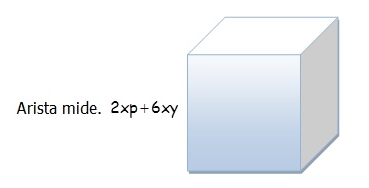
\includegraphics[width=0.4\textwidth]{vic_14.jpg} 
%\end{flushleft}
%\centering\captionof{figure}{Pregunta \ref{vic-14}}\label{fig:vic-14}
%\justifying

\item Se desea construir en el colegio un estanque para el estudio de especies acuáticas en la materia de Biología, si se sabe que  la expresión que representa el arista mide 2xp + 6xy, los estudiantes desean saber ¿Cuál de las siguientes les permitirá calcular el volumen total que ocupara el estanque? (Volumen del cubo es: Lado$^3$)\label{vic-14}


\begin{enumerate}[(A)]
\item $8x^{33}+72x^{32}y+213x^3y^2+216x^3y^3$
\item $8x^3p^3+72x^3p^2y+216x^3py^2+312x^3y^3$
\item $x^3p^3+x^3p^2y+x^3py^2+x^3y^3$
\item $216x^3+32py^2+16x^2yp^2+8p^3$
\end{enumerate}

\item Un almacén de televisores cuenta con 900 televisores de la marca A y 825 de marca B. Se debe distribuir todos los computadores en diferentes compañías de tal manera que todas reciban igual número de televisores marca A y todas reciban igual número de televisores marca B, el número máximo de compañías a las que se les puede hacer la distribución es:\label{vic-15}

\item En un hospital se a determinado que al enfermo lo visita la mamá todos los días, el papa día de por medio, una hermana cada 5 días, un hermano cada 15 días y una tía cada 18 días. Si para el 1 de enero con motivo del año nuevo se encontraron en el hospital, entonces la próxima fecha que se volverán a encontrar sabiendo que febrero tendrá 28 días es: \label{vic-16}

\begin{enumerate}[(A)]
\item 25
\item 75
\item 90
\item 180
\end{enumerate}

\item La siguiente tabla muestra las calificaciones obtenidas por un grupo de estudiantes universitarios, que se presentaron a un examen. \label{vic-17}


\begin{center}
\begin{tabular}[c]{|c|p{3cm}|}
\hline 
Calificaciones & Número de estudiantes  \\ 
\hline \hline
1 & 2	 \\ 
2 & 6 \\  
3 & 18 \\  
4 & 10 \\  
5 & 4 \\ 
\hline 
\end{tabular} 

\end{center}
¿Cuál es la gráfica que representa  la tabla de datos mostrada con  las calificaciones obtenidas?

\begin{enumerate}[(A)]
\item 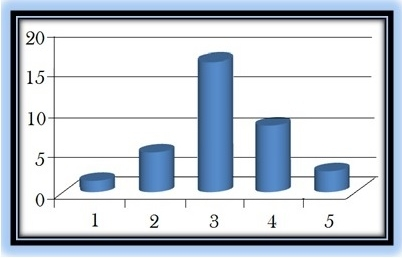
\includegraphics[width=0.3\textwidth]{vic_17_a.jpg} 
\item 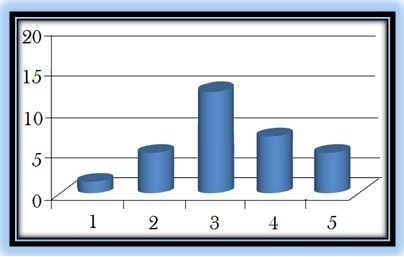
\includegraphics[width=0.3\textwidth]{vic_17_b.jpg} 
\item 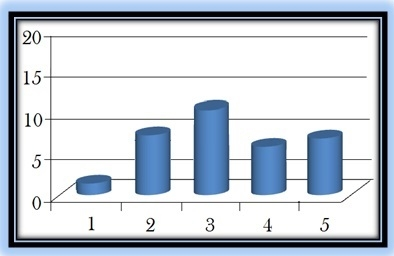
\includegraphics[width=0.3\textwidth]{vic_17_c.jpg} 
\item 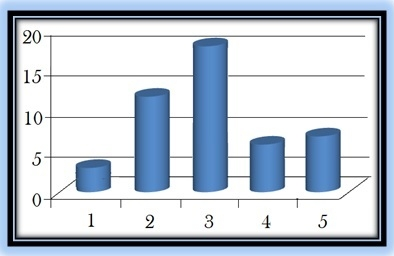
\includegraphics[width=0.3\textwidth]{vic_17_d.jpg} 
\end{enumerate}


\item  En un colegio de Bogotá hay 180 estudiantes repartidos por cada curso como se muestra en la tabla.\label{vic-18}

\begin{center}
\begin{tabular}{|c|cc|}
\hline 
 & Niñas & Niños \\ 
\hline \hline 
Primero & 30 & 15 \\ 
Segundo & 25 & 20 \\ 
Tercero & 27 & 18 \\ 
Cuarto & 33 & 12 \\ 
\hline 
\end{tabular} 
\end{center}


 Si se elige un estudiante al azar, ¿Cuál(es) de las siguientes proposiciones es (son) verdadera(s)?  
 \begin{enumerate}[I]
 \item I La probabilidad de que sea un niño es de $\frac{65}{180}$
\item La probabilidad de que se un estudiante de tercero es  $\frac{45}{180}$
\item La probabilidad de que sea una niña y de segundo es  $\frac{20}{45}$. 
 \end{enumerate}
\begin{enumerate}[(A)]
\item Sólo I
\item Sólo II
\item Sólo I y II
\item Sólo II y III
\end{enumerate}

 \item Tres personas practican natación diariamente de la siguiente forma:\label{vic-19}
Alejandro practica $2\frac{1}{2}$ horas, Patricia $3\frac{1}{4}$ horas y Ricardo $4\frac{3}{4}$ horas. 
¿Cuánto tiempo más práctico  Ricardo que Alejandro?

\begin{enumerate}[(A)]
\item 2 horas.
\item $2\frac{3}{8}$ horas.
\item 3 horas.
\item $2\frac{1}{4}$ horas.
\end{enumerate}
\newpage
\item Se quiere empacar 24 canicas rojas, 36 canicas azules  y  28  canicas amarillas  de tal forma que cada paquete contenga el mismo número de canicas de cada color. El número mínimo de paquetes que se necesita para realizar este empaque es:\label{vic-20}

\begin{enumerate}[(A)]
\item 24
\item 36
\item 6
\item 4
\end{enumerate}

\item Diana tiene contrato para vender azúcar al detal, en kilos (en dos bolsas), las ventas se incrementan diariamente de la siguiente manera progresiva: 8, 18, 28$\cdots$  \label{vic-21}

Al pasar un mes, y si el ritmo de las ventas no cambia, Diana puede decir que venderá cuantos kilos de azúcar:\hrulefill\\
\_\hrulefill\\
\_\hrulefill\\



\item Observa y analiza las siguientes gráficas:\label{vic-22}

%\begin{flushleft}
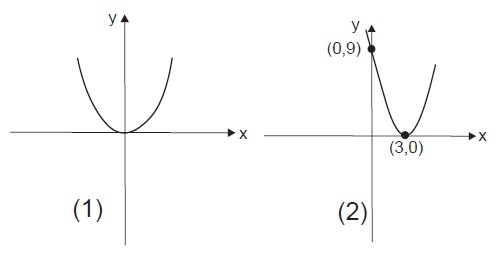
\includegraphics[width=0.45\textwidth]{vic_22.jpg} 
%\end{flushleft}
%\centering\captionof{figure}{Pregunta \ref{vic-22}}\label{fig:vic-22}
%\justifying

De acuerdo con las gráficas anteriores, se podría afirmar que, la gráfica (2) corresponde a la función:

\begin{enumerate}[(A)]
\item $y=x^2-3$
\item $y=x^2+3$
\item $y=(x+3)^2$
\item $y=(x-3)^2$
\end{enumerate}

\newpage
\item  Respecto a las gráficas de las funciones que se presentan a continuación se puede afirmar que: \label{vic-23}

%\begin{flushleft}
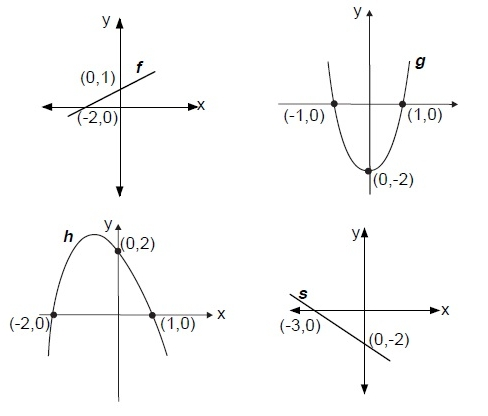
\includegraphics[width=0.45\textwidth]{vic_23.jpg} 
%\end{flushleft}
%\centering\captionof{figure}{Pregunta \ref{vic-23}}\label{fig:vic-23}
%\justifying

\begin{enumerate}[(A)]
\item Las funciones $f$ y $h$ interceptan al eje $y$ en el punto $(0, -2)$.
\item  Las funciones $g$ y $s$ interceptan al eje $x$ en el punto $(-2, 0)$.
\item  $f(1) = s(1) = 0$
\item $g(1) = h(1) = 0$ 
\end{enumerate}
\newpage
\item Observe la siguiente serie de igualdades: \label{vic-24}
\begin{align*}
&1+3=4\\
&1+3+5=9\\
&1+3+5+7=16\\
&1+3+5+7+9=25\\
&\vdots\\
&1+3+5+7+9+\cdots +(2n-1)=¿?
\end{align*}
Si $n$ es cualquier número natural, la suma $1+3+5+7+9+\cdots +(2n-1)$
es igual a: 
\begin{enumerate}[(A)]
\item $n^2$
\item $(2n-1)^2$
\item $(2n)^2$
\item $(n+1)^2$
\end{enumerate}


\newpage
\item En el sistema de coordenadas cartesianas que se muestra en la siguiente figura, se ha representado la trayectoria parabólica del salto de una rana. El desplazamiento horizontal que alcanza la rana en un salto es de 3 metros y la altura máxima es de 1 metro. \label{vic-25}

%\begin{flushleft}
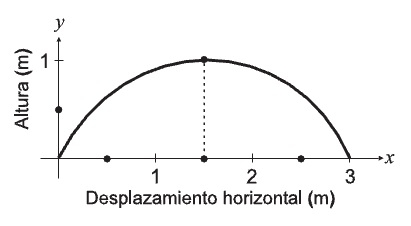
\includegraphics[width=0.45\textwidth]{vic_25.jpg} 
%\end{flushleft}
%\centering\captionof{figure}{Pregunta \ref{vic-25}}\label{fig:vic-25}
%\justifying

La ecuación que describe la trayectoria  del salto de la rana es:

\begin{enumerate}[(A)]
\item $y=-\left (x+\frac{3}{2}\right )^2+1$
\item $y=-\left (x-\frac{3}{2}\right )^2+1$
\item $y=-\frac{2}{3}x-\frac{5}{3}$
\item $y=-\frac{4}{9}x^2+\frac{4}{3}x$
\end{enumerate}

%%%%%%%%%%%%%%%%%%%%%%%%%%%%%
\end{enumerate}
%%%%%%%%%%%%%%%%%%%%%%%%%%%%%5
